% THIS IS SIGPROC-SP.TEX - VERSION 3.1
% WORKS WITH V3.2SP OF ACM_PROC_ARTICLE-SP.CLS
% APRIL 2009
%
% It is an example file showing how to use the 'acm_proc_article-sp.cls' V3.2SP
% LaTeX2e document class file for Conference Proceedings submissions.
% ----------------------------------------------------------------------------------------------------------------
% This .tex file (and associated .cls V3.2SP) *DOES NOT* produce:
%       1) The Permission Statement
%       2) The Conference (location) Info information
%       3) The Copyright Line with ACM data
%       4) Page numbering
% ---------------------------------------------------------------------------------------------------------------
% It is an example which *does* use the .bib file (from which the .bbl file
% is produced).
% REMEMBER HOWEVER: After having produced the .bbl file,
% and prior to final submission,
% you need to 'insert'  your .bbl file into your source .tex file so as to provide
% ONE 'self-contained' source file.
%
% Questions regarding SIGS should be sent to
% Adrienne Griscti ---> griscti@acm.org
%
% Questions/suggestions regarding the guidelines, .tex and .cls files, etc. to
% Gerald Murray ---> murray@hq.acm.org
%
% For tracking purposes - this is V3.1SP - APRIL 2009

\documentclass{acm_proc_article-sp}

\begin{document}

\title{Metadata Extraction from Scientific Literature Using Bidirectional LSTMs
}

\numberofauthors{1} 
\author{
\alignauthor
Molly McMahon\\
       \affaddr{University of Massachusetts Amherst}\\
       \affaddr{140 Governors Dr., Amherst, MA 01003}\\
       \email{mmcmahon@cs.umass.edu}
}

\date{11 May 2017}


\maketitle
\begin{abstract}
TODO
\end{abstract}


\section{Introduction}

Digital libraries provide a variety of services which allow for efficient access to the ever-growing body of scientific literature. The efficacy of research tools such as search, citation indexing, citation and authorship graphs, paper similarity measures, etc. is dependent on the availability and quality of publication metadata. This metadata includes header information, such as title, authors, abstract, affiliations, venues, and dates, as well as bibliographical information and in-text references. However, given the variation in formatting and paper structure that occurs between scientific disciplines and venues, automatic extraction is a difficult task. Extraction tools targeted towards a certain body of literature may produce poor quality results when applied to documents from a different scientific field, or “noisy” unpublished documents. Additionally, formats like PDF do not encode document structure or text formatting information; these text features must be reconstructed using heuristic approaches. As a result, metadata is often flawed or incomplete. In this paper, we address the problem of extracting header metadata from biomedical manuscripts, focusing specifically on token-level classification of pre-extracted PDF text. We focus on labeling paper titles, abstracts, authors, and affiliations, though future work may include citation extraction and parsing. While previous solutions to this problem used models like conditional random fields and SVMs, we propose a deep learning approach. Specifically, we train a bidirectional LSTM (BiLSTM) using the GROTOAP2 dataset, comparing its performance to a logistic regression baseline, as well as a single-layer perceptron. 

\section{Background and Related Work}
There are a variety of existing systems and publications, both open-source and proprietary, which address the problem of metadata extraction from scientific literature. Some tools focus on specific types of metadata, such as header fields or citation parsing, while others provide functionality to extract all metadata types, as well as keywords and other relevant information. While some approaches use heuristic or rule-based techniques to identify specific sections or pieces of metadata, most tools employ some form of machine learning. These tools are trained and evaluated on a variety of datasets, which vary in both discipline (Physics, Mathematics, Computer Science, Biology, Quantitative Finance and Statistics), and size. 

\subsection{Text Extraction and Page Segmentation}
In general, the first step in the metadata extraction process is the extraction of raw text from the existing publication format. The most common format for storing digital manuscripts is PDF. There are numerous utilities which perform text extraction from PDFs, including PDFtoText, Nuance OmniPage, Rexa1-pstotext, PDFBox, PDFMiner, and XPDF. In addition to raw text, some of these tools provide positional information for characters. As the PDF format provides no information about document structure, units such as lines, paragraphs, sections, and headers must be reverse-engineered based on heuristics like spacing, text orientation, and character height. Several algorithms have been devised for this purpose. The recursive XY-Cut algorithm \cite{sutheebanjard2010modified} constructs a hierarchical representation of a document page by recursively subdividing it into smaller rectangular regions using horizontal and vertical cuts. Modified versions of recursive XY-Cut are used to extract blocks of text from PDFs and to establish correct reading order. The Docstrum algorithm is an alternative method for recovering the document structure. It is based primarily on distance between characters and text orientation. \cite{luong2012logical}

Typically, the page segmentation stage yields a hierarchical representation of a document consisting of nested units like individual characters, words, lines, zones, and pages. Using this representation, models may be trained for classification tasks of varying granularity, ranging from word-level labeling (similar to POS tagging and other sequence labeling tasks) to line-level labeling, or in some cases zone-level labeling. Our work focuses on this stage of the extraction pipeline. Existing approaches for labeling and extracting metadata are described in the next section.

\subsection{Metadata Labeling and Extraction}
A variety of models and systems exist to identify, label, and extract different types of metadata information from documents. Some approaches use only heuristic information. For example, SciPlore Xtract \cite{beel2010sciplore} uses font size and style information in a rule-based approach to identify the title of a scientific manuscript. Another open-source system, pdf-extract [3], uses a combination of visual formatting information (such as indentation and spacing) and content-based information (punctuation, prevalence of proper nouns in a text block, etc.) to identify meaningful regions of the PDF, such as the header and the references section. 

While the former rule-based approaches do not require training complex models, machine learning approaches are more prevalent and generally more effective for the task. A multi-stage, “cascading” approach to model training is common among several systems, whereby a coarse-grained model is trained to classify large text regions of the PDF by their roles, and subsequent models are trained to apply finer-grained metadata labels to lines and words within different types of regions. CERMINE and GROBID, described later, both take this approach.

Han, et. al. \cite{han2003automatic} use SVMs with text-based features to classify each line of a paper header into one of 15 classes. They iteratively improve the initial labeling of each line by considering the labels applied to adjacent lines until a “convergence” is reached. Following line-level classification, chunking is applied within lines for finer-grained metadata extraction, such as recognizing individual authors in multi-author lines. Kovačević et. al. \cite{kovavcevic2011automatic} use eight SVMs with formatting, positional, and word features to classify lines of text into eight categories. CERMINE \cite{tkaczyk2015cermine}, an open-source system for PDF metadata extraction, uses a two-stage SVM approach to classify zones (or multi-line blocks) of text into different metadata classes. In the first stage, each zone is classified into one of four coarse-grained classes - metadata, body, references, or other. In the second stage, metadata zones are further classified into finer-grained metadata categories (title, author, abstract, etc.) using another SVM. The features used for zone classification include geometric features (zone width, height, and positioning), lexical features (dictionary word-matching), sequential features (labels and attributes of adjacent zones), formatting features (font and whitespace), and heuristic features (line casing, digits, etc.).

In addition to SVMs, Hidden Markov Models (HMMs) and Conditional Random Fields (CRFs) have widely studied for the task of scientific metadata extraction. Peng, et. al. [10] use CRFs with text, layout, and dictionary based features to extract information from PDFs, investigating the effects of model regularization and priors. Their approach achieves a higher F1 score for most fields when compared to previous HMM or SVM models. GROBID \cite{lopez2009grobid} uses 11 CRF models, following the cascading model approach described earlier. Using positional features, lexical features, and layout features, GROBID segments the document into cover, header, body, footnotes, headnotes, bibliography, and annex sections. Within these sections, additional CRFs are used to further segment the text into finer-grained metadata classes. Along with header metadata and document text, GROBID identifies and parses the reference strings contained in the document’s bibliography. CERMINE also performs extraction and parsing of reference strings from the reference zones of the PDF, using K-Means clustering to identify individual references and CRFs to parse the metadata fields of each reference. ParsCit \cite{councill2008parscit}, a system specifically for parsing reference strings, uses CRFs to label and segment the words in each citation. SectLabel \cite{luong2012logical}, an extension of ParsCit, uses CRFs to capture a document’s logical structure (including sections and subsections, tables, figures, equations, footnotes, and captions, along with title, authors, and references). The system consists of a “Logical Structure” module, which takes in the full text and labels lines according to logical role, and a “Generic Section” module, which takes header lines as input and applies metadata labels to the lines. 

It is difficult to determine which of the previously mentioned tools is the “state-of-the-art” for metadata extraction, as the models were trained and evaluated on different datasets, apply labels at varying levels of granularity (line, word, and zone), and target different classes of metadata (header fields, citation strings, etc.). However, Lipinski et. al. \cite{lipinski2013evaluation} provide an evaluation of six tools - GROBID, Mendeley Desktop, ParsCit, PDFMeat, PDFSSA4MET, SciPlore Xtract, and SVMHeaderParse - on a dataset of 1,153 random PDFs collected from arXiv. These documents span the fields of Physics, Mathematics, Computer Science, Quantitative Biology, Quantitative Finance and Statistics. The tools were compared in terms of their accuracies for title, authors, author last name, abstract, and year fields; partial points were given for partially correct results, as determined both manually and by Levenshtein distance. Based on their experiments, GROBID performed the best overall, achieving scores of 0.92 for titles, 0.83 for authors, 0.91 for authors’ last names, 0.74 for abstracts, and 0.69 for publication date.

The authors of CERMINE also provide a detailed evaluation, in which they compare the precision, recall, and F scores of several systems to that of CERMINE, using a test set comprised of 1,943 PubMed Central articles with associated metadata. Of the evaluated systems, CERMINE achieved the best F1 score on almost all metadata types. This may be because CERMINE was trained on a dataset comprised of PubMed PDFs, while the other systems were trained using data from other domains.


\subsection{Deep Learning for Structured Prediction}
Deep learning techniques have been employed for a variety of natural language processing tasks. Despite their demonstrated efficacy on other NLP problems, it does not appear that any deep learning approaches have been leveraged for the specific problem of metadata extraction. However, metadata extraction may be viewed as a case of structured prediction, a problem for which deep learning techniques have been widely and successfully employed. Common instances of structured prediction include sequence tagging (e.g. part-of-speech tagging), sequence segmentation (e.g. chunking and named entity recognition), and syntactic parsing - of these, metadata extraction is most similar to NER. \cite{goldberg2016primer}

Various neural architectures have been applied to the problem of structured prediction. Many of these approaches are designed to skirt the need for labor-intensive, task-specific feature engineering. For example, Collobert et al. \cite{collobert2011natural} describe a convolutional neural network (CNN) architecture designed to excel on multiple benchmark tasks by learning more general internal representations “from scratch.” Using word embeddings, along with a few additional features like dictionary prefix matching and capitalization schemes, they create an “all-purpose” tagger which performs competitively on POS tagging, chunking, NER, and semantic role labeling benchmarks. However, feed-forward networks can only capture a limited amount of context, dependant on the size of the context window. In this respect, recurrent neural network (RNN) architectures have an advantage over feed-forward networks, as they can more effectively capture long-distance dependencies between words. RNNs also differ from feed-forward networks in that they “have memory”; the outputs from previous timesteps are considered when making a decision for the current timestep in a sequence. Thus, in addition to CNNs, a variety of RNN architectures have been used for sequence labeling tasks. In particular, bidirectional LSTMs (BiLSTMs) have produced state-of-the-art results for POS tagging, chunking, and NER. BiLSTMs are a specific variety of Bidirectional RNNs first employed by Graves, et. al. for speech recognition. \cite{graves2013hybrid} Chiu, et. al. use a hybrid BiLSTM-CNN architecture to automatically detect word and character features for NER. \cite{chiu2015named} Their network uses word embeddings trained by Collobert, et. al. alongside character embeddings learned using a CNN, as well as additional word features like capitalization and lexicon matching. Their lexicon matches are defined using a novel scheme involving partial prefix and suffix matching, as well as BIOLU annotation of each token in a dictionary match. Using a BiLSTM-CNN augmented with their improved lexicon matching scheme, they were able to obtain new state-of-the-art results on CoNLL-2003. Huang, et. al. performed a comparison of LSTMs, BiLSTMs, LSTM-CRFs, and BiLSTM-CRFs for the Penn Treebank POS set and CoNLL 2003 chunking and NER sets, using both embeddings and hand-engineered word features. \cite{huang2015bidirectional} Adding a CRF on top of an LSTM architecture enables the network to efficiently use sentence-level tag information, such that the optimal tag sequence may be computed using dynamic programming. The BiLSTM-CRF outperformed all baseline models, and was able to achieve good performance even when the hand-engineered features were removed. Ma, et. al. take a similar approach, but include a CNN to extract character features, producing a hybrid BiLSTM-CNN-CRF architecture that uses no additional lexicon matching or feature engineering. \cite{ma2016end} With their network, they set new state-of-the-art performances on the Penn Treebank WSJ POS tagging corpus and the CoNLL 2003 NER corpus. Lample, et. al. train both a BiLSTM-CRF and an LSTM using a “transition-based approach inspired by shift-reduced parsers” to label sequences, achieving state-of-the-art NER results across four languages without the use of lexicon matching or language-specific features. \cite{lample2016neural}

\section{Model}
Much of the prior work related to metadata extraction focuses on applying metadata labels to lines or zones of text. However, this approach is insufficient in cases where a line or zone contains multiple classes of metadata; for example, a zone of text may contain alternating lines of authors and affiliations, or a line may contain an author’s name followed by the author’s affiliation. Rather than taking the “cascading model” approach and training additional models for token-level classification within specific zones, we frame metadata extraction as a generic sequence labeling task; specifically, we aim to directly classify individual tokens, in a manner similar to part-of-speech tagging or named entity recognition (NER). 

\subsection{Bidirectional LSTMs for Sequence Tagging}
Long short-term memory networks (LSTMs) are a variety of recurrent neural networks (RNNs) designed to capture long-range dependencies within sequences. While simple RNNs can be difficult to train due to vanishing gradients during backpropagation, LSTMs incorporate special “memory cells” composed of gating components to preserve gradients over many time steps. \cite{goldberg2016primer} A “gate” consists of a vector of values in the range [0,1] passed through a sigmoid, which is multiplied point-wise with another vector, only allowing certain information to “pass” through. These gates control how much information is preserved in the memory cell state at each time step by allowing the  network to “forget” previously learned information. The following is the mathematical definition of an LSTM unit:
\begin{equation}
    i_{t}=\sigma(W_{xi}x_{t}+W_{hi}h_{t-1}+W_{ci}c_{t-1}+b_f)
\end{equation}
\begin{equation}
    f_t=\sigma(W_{xf}x_{t}+W_{hf}h_{t-1}+W{cf}c_{t-1}+b_f)
\end{equation}
\begin{equation}
    c_t=f_tc_{t-1}+i_t\tanh(W_{xc}x_t+W_{hc}h_{t-1}+b_c)
\end{equation}
\begin{equation}
    o_t=\sigma(W_{xo}x_t+W_{ho}h_{t-1}+W_{co}c_t+b_o)
\end{equation}
\begin{equation}
    h_t=o_t\tanh(c_t)
\end{equation}

Here, $x$ is the input sequence ($x_1,....,x_T$). $f$ is the forget gate vector, $i$ is the input gate vector, $c$ is the cell state vector, $o$ is the output gate vector, and $h$ is the hidden state vector, all at timestep $t$. $W$ and $b$ correspond to weights and biases for each layer. \cite{graves2013hybrid} $\sigma$ refers to the logistic sigmoid function. (TODO include diagram of LSTM unit if necessary?)

Bidirectional LSTMs are a variant of LSTMs which consider information from both past and future inputs at a given point in a sequence. The network includes both forward and backward hidden states at each timestep, which are combined to compute the output for each timestep, as specified by Graves et. al:

\begin{equation}
    \overrightarrow{h_t} = \mathcal{H}(W_{x\overrightarrow{h}}x_t+W_{\overrightarrow{h}\overrightarrow{h}}\overrightarrow{h}_{t-1}+b_{\overrightarrow{h}})
\end{equation}
\begin{equation}
    \overleftarrow{h_t} = \mathcal{H}(W_{x\overleftarrow{h}}x_t+W_{\overleftarrow{h}\overleftarrow{h}}\overleftarrow{h}_{t-1}+b_{\overleftarrow{h}})
\end{equation}
\begin{equation}
    y_t=W_{\overrightarrow{h}y}\overrightarrow{h}_t+W_{\overleftarrow{h}y}\overleftarrow{h}_t+b_y
\end{equation}
Here, $\mathcal{H}$ refers to an element-wise sigmoid function. $\overrightarrow{h}_t$ is the forward hidden state, computed by iterating over the input from timestep 1 through $T$, and $\overleftarrow{h}_t$ is the backward hidden state, computed by processing the input from timestep $T$ through 1. $y_t$ is the output at time $t$. \cite{graves2013hybrid} Figure 1 shows a BiLSTM which takes as input a sequence of token feature vectors, each composed of word embeddings, character features, and additional features.
\begin{figure}[h]
\caption{Bidirectional LSTM for Sequence Tagging}
\centering
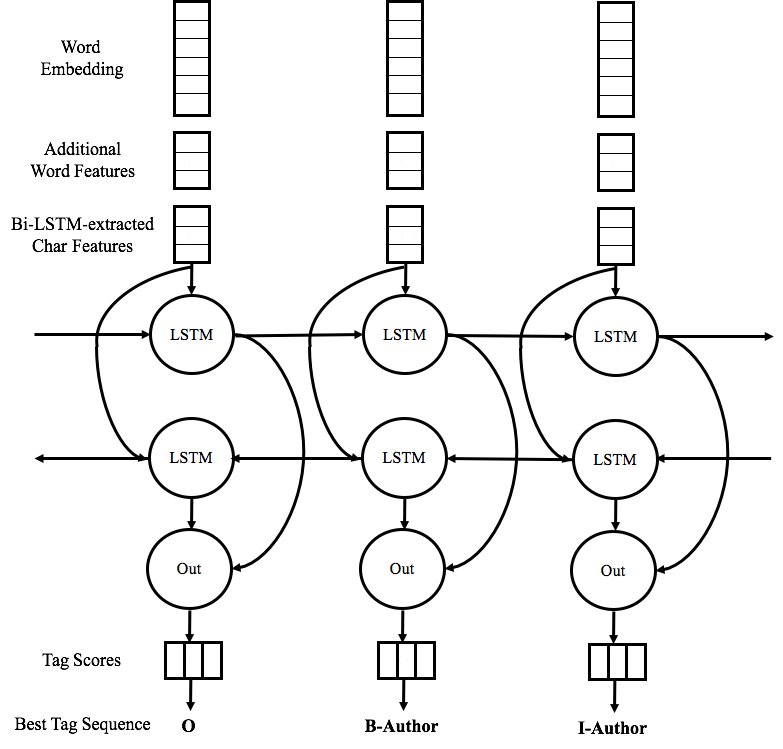
\includegraphics[width=0.5\textwidth]{bilstm.png}
\end{figure}
In the case of metadata extraction, our input sequences consist of words and word-related features extracted from a PDF document using one of the previously described techniques. We use a BiLSTM to process these word sequences, outputting the appropriate metadata label for each word in the document. Our implementation of the output layer varies slightly from that described by Graves, et. al. We concatenate the forward and backward hidden layers, pass the result through a $tanh$ layer, then through a final output layer to obtain the scores.

\subsection{Bidirectional LSTM For Character Feature Extraction}
In addition to word-level features, we also extract character-level features for each word in the document. These are added to the input sequence along with the other features. This is similar to the approach taken by Chiu et. al., but rather than a CNN, we use an additional BiLSTM network to perform this feature extraction. We treat the hidden layer dimensions and output dimensions as hyperparameters.

\section{Experiments}
\subsection{Dataset}
To train our models, we use the GROTOAP2 (GRound Truth for Open Access Publications) dataset, which consists of 13,210 ground truth articles from PubMed Central, spanning 208 different publishers. \cite{tkaczyk2014grotoap2} This dataset was used to train the models in the CERMINE metadata extraction system. Each document in the dataset is represented using the TrueViz format, an XML-like format which encodes the document structure. TrueViz represents the document as a hierarchy. A document consists of a list of pages, pages consist of lists of zones, zones consist of lists of lines, lines consist of lists of words, and words consist of lists of characters. Words, lines, and zones all include bounding box information, which establish their height, width, and location on the XY plane beginning in the top-left corner of the page. TrueViz also encodes the reading order and the metadata labels of all zones in the document. Each zone is assigned one of the following 22 labels:

\begin{itemize}
\item abstract 
\item acknowledgments 
\item affiliation
\item author
\item bib\_inf
\item body\_content 
\item conflict\_statement 
\item copyright 
\item correspondence
\item dates 
\item published dates
\item editor
\item equation 
\item figure 
\item glossary
\item keywords
\item page number
\item references
\item table
\item title 
\item title\_author 
\item type 
\item unknown 
\end{itemize}
As this dataset was created semi-automatically, the labeling is not completely accurate; based on a random sample of 100 documents from the dataset, the authors estimate the overall accuracy of the annotation to be about 93\%. They deem this level of accuracy sufficient to train useful models. Of the given labels, we focus on identifying title, author, abstract, and affiliation - the rest of the labels may simply be considered as “other.”

We use only a subset of the dataset to train our models. Our training set consists of 2,518 documents and our test set consists of 1,452 documents. We originally aimed to expand our train, test, and development sets to include all 13,000 documents in the GROTOAP2 set, but due to time constraints related to training and tuning, this was not feasible.

\subsection{Data Representation and Features}
For our experiments, we take all the words on a the first page of a document, arranged in their correct reading order, and segment the page into word sequences of length 30. Each word is assigned the label of its enclosing zone, using BILOU encoding. We chose to define example sequences in this manner for several reasons. Firstly, the dataset is labeled at the zone level. Therefore, taking a line or a zone as an example would yield a sequence with only one type of metadata label; a model trained on these types of examples would not learn to distinguish between different metadata types occurring on the same line, rendering the word-level classification useless. By slicing the document into example sequences of 30 contiguous words which may span multiple lines and zones, we define examples that may include more than one metadata type. The maximum length of 30 was determined somewhat arbitrarily - we originally aimed to use an entire page as a training sequence, but this approach was too memory-intensive to be feasible. 

Unlike traditional sequence labeling tasks, there are specific visual cues such as page layout, font size, and indentation, which may be informative of a word’s metadata label. These features must also be incorporated into a word’s representation to obtain the best results. The word-level features we extract from the GROTOAP2 documents can be divided into five categories: word embeddings, word shape, geometrical features, character features, and dictionary features. Continuous values are rescaled to the range [0,1], and binary or categorical features are embedded into a 5-dimensional vector space, using the approach described by Collobert, et. al. for encoding additional word features. \cite{collobert2011natural}

\subsubsection{Word Embeddings}
In our embedding lookup layer, we use pre-trained embeddings specific to the biomedical domain. Moen, et. al. provide several sets of 200 dimension word embeddings trained with word2vec on texts from PubMed Central, PubMed, and an English Wikipedia text dump. \cite{moen2013distributional} These embeddings files are large, with the smallest set containing around 2.5 million word embeddings. The majority of these words do not occur in our dataset, or occur only rarely - therefore, in the interest of memory, we load only embeddings for words with 10 or more occurrences in the dataset. Words that occur less than 10 times are considered out-of-vocab (OOV). After applying this pruning to the PMC word2vec file, we were left with about 600,000 words, which cover about 85\% of the words that occur in the training and test data.

\subsubsection{Word Shape}
For each word, we encode one of four word shapes into our feature vectors, based on the word’s pattern of capitalization. The possible word shapes are all-caps (AAA), lowercase (aaa), capitalization followed by lowercase (Aaa), and a mix of lowercase and capital letters (aAa). These shapes are then embedded into a 5-dimensional space - the shape feature vectors are learned by the network at training time.

\subsubsection{Geometrical Features}
We include several features related to the dimensions of word bounding boxes, namely the word width, word height, and width-to-height ratio. We also include the X and Y coordinates of the centerpoint of the word bounding box to capture where the words occur on the page. Each coordinate is represented as a percentage, indicating where it falls within the range defined by the minimum and maximum coordinate on the page. We also include line and zone ids (represented as a percentage of the largest line and zone ids on a page) with the intent of capturing the word’s position in the overall reading order of the document, as this may differ from its XY position.

\subsubsection{Character Features}
In order to capture character-level features, we train 25-dimensional character embeddings using an additional BiLSTM with 30-dimensional hidden layers. 

\subsubsection{Dictionary Matching Features}
With the intent of improving the labeling of words that are likely to be OOV, such as author names or affiliations, we include several dictionaries membership features. We assembled four dictionaries - a places dictionary, a person\_names dictionary, a department dictionary, and a university dictionary. The places dictionary includes common city, region, and country names. The person\_names dictionary includes common first and last names in English, Chinese, and other languages. The department dictionary includes words that often occur in department names, such as “institute” and “college”. The university dictionary includes the names of universities. For each token in an example sequence, a partial match is computed between the token and the contents of each of the dictionaries. For each dictionary, we have a binary feature which is set to 1 if the token matches any words in a dictionary with a cosine similarity of 0.9 or greater. For each of these binary features, a 5-dimensional embedding is learned.

\subsection{Training and Evaluation}
Our training scheme was similar to that used by Strubell, et. al. \cite{strubell2017fast} Using the GROTOAP2 subset and feature representation described above, we trained a BiLSTM network with a hidden LSTM dimension of 150, using minibatch stochastic gradient descent with a batch size of 64 and an adaptive learning rate using the Adam update rule. \cite{kingma2014adam} To reduce overfitting, we used L2 regularization and dropout on each network layer, as well as word dropout for learning a representative OOV word embedding. \cite{lample2016neural} Our layer weights were initialized using Xavier initialization \cite{glorot2010understanding}. In addition to the BiLSTM, we trained a logistic regression model, and a single-layer perceptron network with a hidden layer of 210 ReLU units. Both the logistic regression and perceptron models used lexical and geometrical features similar to the BiLSTM, and incorporated features from the target token’s 8 neighboring tokens in an attempt to incorporate contextual information. Models were evaluated based on their overall per-token accuracy and weighted F1 scores, as well as the precision, recall, and weighted F1 for each of the labeled fields (disregarding BILOU and using only raw labels, as our baseline models do not use BILOU encoding). 

Table [number] summarizes the hyperparameter settings used to train all BiLSTM models. These hyperparameters were selected using a grid search over various combinations of dropout, learning rate, Adam beta and epsilon, hidden layer dimension, regularization penalty, and batch size settings. We trained a model for each combination, iterating over the training set until there were no significant changes in the loss between epochs (in other words, until the loss had “converged”). We selected the hyperparameter settings which yielded the best weighted F1 score on the development set. The final model was trained for 30 epochs.


\section{Results and Discussions}
Table [number] shows a comparison of the models’ performances on the test set. For all labels, the neural network models far outperformed the logistic regression baseline. While for most fields, the BiLSTM outperformed the perceptron, the BiLSTM’s recall for the Title field was notably poor. The reason for this poor performance is unclear; it is possible that the BiLSTM was not placing sufficient weight on geometrical features such as text positioning or line height. Inspection of the confusion matrix indicates that Title was often mislabeled as Other, which may also account for the BiLSTM’s subpar precision for Other. Due to time constraints, we were unable to search a large space of hyperparameters for the neural network models - a more effective tuning scheme over a wider range of hyperparameters, perhaps using random search instead of grid search, may have yielded better models and made the BiLSTM and perceptron more distinguishable.

(insert table)

Table [number] compares the performance of the BiLSTM with and without the inclusion of lexicon and geometric features. The BiLSTM-basic model was trained using only word and character embeddings, while the BiLSTM-geo-lex model was trained using word embeddings, character embeddings, and all of the additional geometrical and dictionary-matching features described in Section [number]. The inclusion of geometric information and dictionary matching significantly boosted the overall accuracy and weighted F1 score of the model; in particular, the precision, recall, and F1 for Abstract were dramatically improved. Surprisingly, the Author and Affiliation fields also only slight improvements in precision, recall, and F1. We expected an increase is due to dictionary matching of names and universities that are likely to be out of vocab - however, this increase was not as significant as we expected, which may indicate that our embedding scheme for lexicon matching was ineffective. That the model was able to achieve competitive precision and recall for Author and Affiliation using word and character embeddings alone implies that the model learned a high-quality OOV embedding, or that character embeddings are particularly informative of these fields. Surprisingly, the metrics for the Title field were not significantly improved by the inclusion of geometrical features, indicating that our model may not be properly weighting the geometrical features, or that a bug may exist.


Our results indicate that deep learning approaches show significant improvements over simpler linear models like logistic regression. In particular, the BiLSTM achieves the best performances for most of the fields, though it falters when retrieving the Title field. In addition, the BiLSTM appears to be fairly robust, in that it performs well with little feature engineering - using only word and character embeddings, the basic BiLSTM model still outperforms the logistic regression model on all metrics except Title recall and F1. It is likely that with further tuning and a larger training set, the BiLSTM.

\section{Conclusion and Future Work}
Our experiments confirm the potential usefulness of BiLSTMs for the task of metadata extraction. It is likely that with further tuning and a larger training set, the BiLSTM could be a competitive alternative to existing CRF models. As such, future work for this project may include further experimentation with hyperparameter settings, as well as a more thorough analysis of performance for specific fields. Varying the length of example sequences may also yield increases in performance. In addition, it may be prudent to evaluate F1 on a per-entity basis, rather than on a per-token basis, to facilitate comparison with existing systems and models like CERMINE. Finally, we may explore Dilated Convolutional Neural Networks (Dilated CNNs) as an alternative to the BiLSTM model, as they have been shown to perform competitively on sequence labeling tasks and train more quickly than LSTM models. \cite{strubell2017fast}

\section{Acknowledgements}
I would like to thank Emma Strubell for her guidance and the use of her cnn-spred code, as well as Shankar Vembu of the Chan Zuckerberg Initiative/Meta for his mentorship this semester. In addition, I would like to thank Sheshera Mysore, Akul Siddlingaswamy, and Aditya Narasimha Shastry, who were my partners for this project; they implemented and trained the logistic regression and perceptron models.

\bibliographystyle{abbrv}
\bibliography{sample}

%\balancecolumns 

\end{document}
